\chapter{Methodology}
The current section concerns the approaches which were made in undertaking this project, what validation was used, and how units of work were tracked during the course of the project.

\section{Requirements Gathering}
Requirements for this project were gathering in chapter~\ref{chap:intro}, the specific sections where the requirements for the application can be found in these sections, \ref{section:objectives}, \ref{section:stack} and \ref{section:idea}

\section{Planned Approach to Project}
The original planned approach to the application can be seen below in the form of a gantt chart.

\begin{figure}[h!]
    \centering
    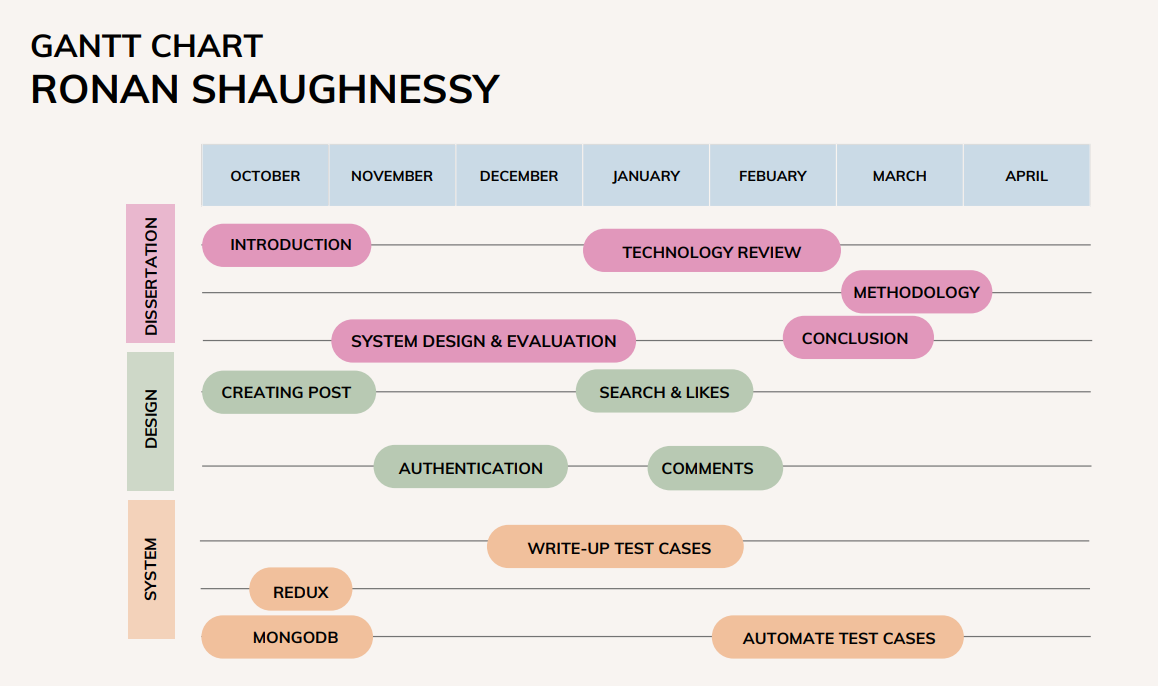
\includegraphics[width=0.5\textwidth]{images/GanttChart.png}
    \caption{Gantt Chart}
    \label{image:GanttChart}
\end{figure}

\newpage
\section{Methodology Approach}
Rather than one single approach, multiple methodologies were used in the creation of the application, Extreme Programming for development, Behaviour Driven Development for testing the application, Jira Software agile tool was also used to track progress alongside GitHub.

\subsection{Extreme Programming}
The approach which was undertaken in order to complete tasks done each week was extreme programming(XP) \cite{akhtar2022extreme}. XP is a agile framework, which takes the agile methodology to the extreme, in short this means shorter sprints combined with more tasks in each sprint. The aims of using XP was to make the most use out of the limited amount of time that was set for the creation of the project, with this in mind maximising all the time during the college year was crucial to the applications success. Lastly XP can handle changes to the requirements smoothly, if the need was deemed high enough for the application.

\subsection{Behaviour Driven Development}
Behaviour Driven Development(BDD) is developing the application, to behave as expected if the application does not function as thought, then work is needed to improve to make the system in order to make it compliant with user behaviour and allow the application to work with ease \cite{abushama2020effect}. BDD was employed to great extent during the testing phases of the application, where test cases needed to be designed based on how the user would interact with the program, in order to assert if it works as planned.

\section{Validation}
Instruments which were used in order to test the application ensuring its appropriate use.

\subsection{White \& Black Box Testing}
Black box methodology was employed using BDD, as BDD takes the role of a user who doesn't care how the applications code base works, only that the application does what is expected. This was used in automated testing of the application, as the Cypress testing tool has no prior knowledge of the internal code base, only simulating user behaviour. White box methodology was employed at a manual test level, as I had a clear idea of the code base which I was working on in order to test the application.

\begin{figure}[h!]
    \centering
    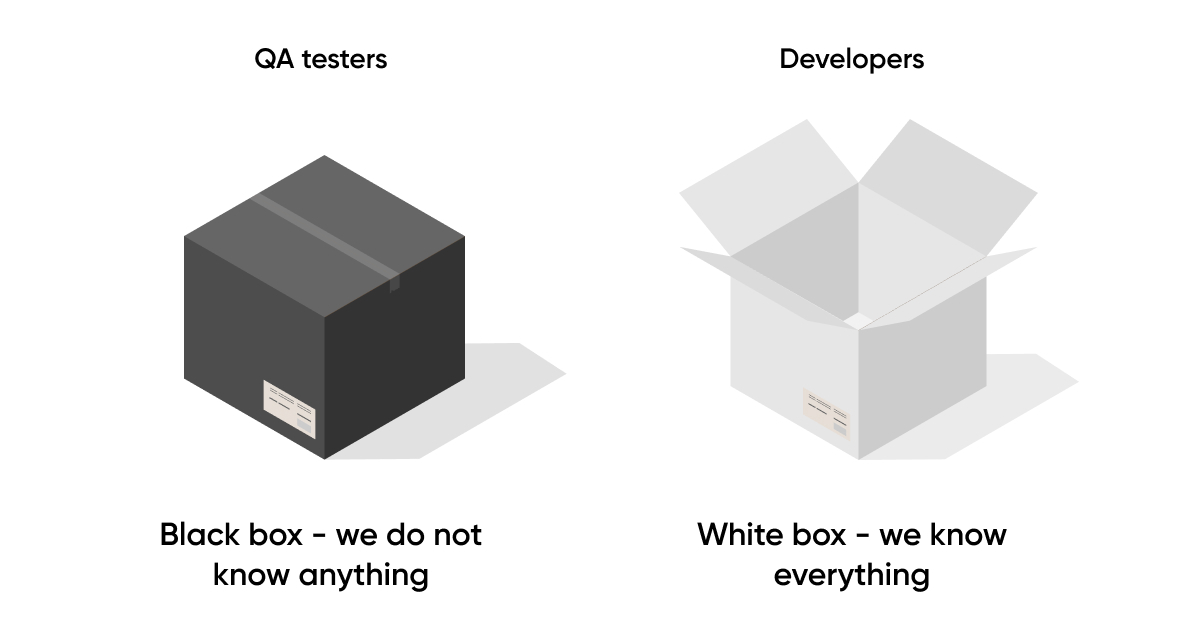
\includegraphics[width=0.5\textwidth]{images/WhiteAndBlack.jpg}
    \caption{White Box vs Black Box Testing}
    \label{image:WhiteAndBlackBox}
\end{figure}

\subsection{Manual Testing}
As previously stated, white box methodology was used during manual testing of the application. When certain restful APIs were called using the application's internal code base, a console.log would be applied to the controller at the back end to determine whether or not there was an error. The aforementioned testing was performed on the application several times throughout the project, using Google's console in the browser to assert if there were errors in the code, this was also accomplished quite successfully with the use of status codes such as the 400, 500 and 200.

\subsection{Automated Testing}
Automated validation was conducted with black box methodology in mind, in which the application would simulate user behaviour for example liking a post once signed in, or creating a post. Automated testing was employed to ensure the front end of the application was working correctly as a user would intend for it to work.

\section{Source Control}
Tools which were used in order to track and manage the software programming.

\subsection{Jira Software}
Jira was used in conjunction with extreme programming to track tickets/tasks. Atlassian stories were created under epics and then brought from the backlog into a new sprint. When a previous sprint finished, tasks were taken into a sprint from the backlog then a new sprint was started, since it was a one man team, each sprint varied in time in custom with XP. At the end of each sprint, the tasks done were evaluated as to how well the aforementioned tasks were completed, after which tickets would be updated if they needed to be brought into the next sprint for improvement, if bugs were found through the use of testing preformed such bugs were logged to be solved in the next sprint, any enhancements which could be made to the application would also be taken into the next sprint.

\subsection{GitHub}
Once a number of tickets were completed during a sprint for example two, then the programming workload would be committed to GitHub, when used in conjecture with Jira it aided to track the projects progress. This was to ensure that the application was always in a stable state, for example if work proceeded after the latest commit, and the code that was being worked on during the latest ticket introduced a breaking bug that halted the application, GitHub could be used to revert the code base, thereby getting the application back to its previous working state. 
